\documentclass[12pt]{amsart}
\pagestyle{empty}
\usepackage[hmargin=1in,vmargin=1in]{geometry}
\usepackage{url,  mathrsfs}
\usepackage{hyperref}
\usepackage{fancyhdr} 
\usepackage[T1]{fontenc}
\pagestyle{fancy}
\fancyhf{} % Clear existing headers and footers

% Example 1: Author name on the left, page number on the right
\fancyhead[L]{Grant Yang - MATH 380 Spring 2026}
\fancyhead[R]{\thepage}

\usepackage{listings,xcolor}
\lstset{language=Mathematica}
\lstset{basicstyle={\sffamily\footnotesize},
  numbers=left,
  numberstyle=\tiny\color{gray},
  numbersep=5pt,
  breaklines=true,
  captionpos={t},
  frame={lines},
  rulecolor=\color{black},
  framerule=0.5pt,
  columns=flexible,
  tabsize=2
}


\usepackage{quiver}

\usepackage{biblatex} %Imports biblatex package
\addbibresource{cite.bib} %Import the bibliography file

\usepackage{url,  mathrsfs}
\usepackage{hyperref}
\usepackage{amsmath}
\usepackage{cancel}
\usepackage{amssymb}
\usepackage{graphicx,  epstopdf}
\usepackage{subfig}
\usepackage{color}
\usepackage{bbm}
\usepackage{subfloat}
\usepackage{float}
\usepackage[draft]{fixme}
\usepackage{bm} 
\usepackage{bbm} 
\usepackage{epigraph}
\usepackage{endnotes}
\usepackage{ifpdf}
\usepackage{array}

\usepackage{multicol}
\usepackage{multirow}
\usepackage{graphicx}
\usepackage{tikz}

\newcommand{\A}{\mathbb{A}}
\newcommand{\Q}{\mathbb{Q}}
\newcommand{\N}{\mathbb{N}}
\newcommand{\Z}{\mathbb{Z}}
\newcommand{\R}{\mathbb{R}}
\newcommand{\F}{\mathbb{F}}
\newcommand{\C}{\mathbb{C}}
\renewcommand{\P}{\mathbb{P}}
\newcommand{\I}{\mathcal{I}}
\newcommand{\V}{\mathcal{V}}
\newcommand{\cH}{\mathcal{H}}
\newcommand{\ol}{\overline}
\newcommand{\J}{\mathcal{J}}
\newcommand{\X}{\mathcal{X}}
\theoremstyle{definition}
\newtheorem{prob}{Problem}
\newtheorem{extraProb}{Extra Problem}

\DeclareMathOperator{\conv}{conv}
\DeclareMathOperator{\cone}{cone}
\DeclareMathOperator{\ext}{ext}




\begin{document}
 \thispagestyle{empty}
\title{Cyclic Error Correcting Codes}
\author{Grant Yang}
\maketitle

\section{Introduction}
When communicating over noisy channels, there is always a chance that the message you send will not perfectly match the message received. To solve this problem, error correcting codes are employed in everything from QR codes to the Voyager spacecraft, used to encode messages into special codewords that allow us to detect and correct flipped bits. Error correcting codes are essentially just schemes for mapping messages to codewords, balancing the tradeoff between resiliency to errors and efficiency--- both in computation for encoding and decoding, and in the size of the codeword to be transmitted.

In this paper, we will be dealing with \emph{block codes}, where we encode each block of $k$ bits (our \emph{message}) into a $n$-bit long \emph{codeword}. In fact, we will be looking specifically at codes that are also \emph{linear} and \emph{cyclic}, a class of codes with nice properties that includes famous schemes such as Hamming codes and Reed-Solomon codes. 

To explain what we mean by linear, note that we can view our messages and codewords as vectors in $\mathbb F_2^k$ and $\mathbb F_2^n$ respectively, where $\mathbb F_2$ is the finite field with two elements, $0$ and $1$. Here, $\mathbb F_2$ is another name for $\mathbb Z/2\mathbb Z$ or $\mathbb Z_2$ (integers mod 2), where addition is bitwise \verb|XOR| and multiplication is bitwise \verb|AND|. One can check that this satisfies the field axioms.\footnote{In general, you can use finite fields with more elements, which we write as $\mathbb F_q$. It turns out that every finite field with $q$ elements is isomorphic, and we only get a field when $q=p^n$ where $p$ is prime and $n \in \mathbb N_{>0}$. These things are also called ``Galois Fields,'' and sometimes people write $\mathrm{GF}(q)$ instead of $\mathbb F_q$.} For our code to be linear, we want the mapping from messages to codewords to be linear: the codeword for $m+m'$ should be the sum of the codewords for $m$ and $m'$. If we were to stop here, we could use a \emph{generator matrix} $G : \mathbb F^k_2 \to \mathbb F^n_2$ and simple linear algebra,\footnote{Actually, it is convention to write this transposed and use row vectors for some reason...} but we also want our codes to be cyclic! We want shifting any codeword (e.g. $wxyz \mapsto xyzw$) to give us another valid codeword, and now it becomes very natural to use polynomial rings, as this shifting operation is exactly multiplication by $x$ in a special kind of \emph{quotient ring}.

\section{The Quotient Ring}
Instead of viewing our message as a vector $m \in\mathbb F_2^k$, we can consider it as a polynomial \[m(x)=m_1 x^{k-1}+m_2x^{k-2}+\dots m_k \in R,\]
where $R$ is our quotient ring $R = \mathbb F_2[x]/\langle x^n - 1\rangle$. Approximately, $R$ is the set of remainders upon division by $x^n-1$, where $n$ is the length of our codewords.

The quotient means that we are working `modulo' this polynomial $x^n-1$, effectively introducing a new relation $x^n \equiv 1$ into our original polynomial ring $\mathbb F_2[x]$. For a simpler analogy, consider $\mathbb Z/2\mathbb Z$, where we take the ring of integers and `quotient out' by the ideal of even integers. We do all our addition and multiplication modulo $2$, and we have effectively introduced the equivalence $2\equiv 0$ into our ring. 

We will avoid the full formal definition of quotients of arbitrary rings by arbitrary ideals, but to get a hint of it, let us review the results of Homework 4, \S2.6 Exercise 13 to get an understanding of $R = \mathbb F_2[x]/\langle x^n -1\rangle$. First, note that since the ideal $\langle x^n - 1\rangle$ is principal (generated by just one element), we have as a Gr\"obner basis simply $G = \{x^n - 1\}$. For any $f,g \in \mathbb F_2[x]$, the homework problem shows that
\begin{enumerate}
    \item $\overline{f}^G = \overline{g}^G \iff f-g \in \langle x^n-1\rangle$.
    \item $\overline{f+g}^G = \overline{f}^G + \overline{g}^G$.
    \item $\overline{\overline{f}^G\overline{g}^G}^G = \overline{fg}^G$.
\end{enumerate}
We can consider $R$ as the set of remainders upon division by $x^n-1$, and one can use these three properties to show that addition and multiplication modulo $G$ make $R$ a ring. Additionally, note that $R$ is finite: it is the set of polynomials with degree at most $n-1$, and finally we can see that multiplication by $x$ in this ring corresponds to a circular shift of our codeword, since $x^n \equiv 1$:
\[(c_1 x^{n-1} + c_2 x^{n-2}+ \dots + c_n) \cdot x =  c_2 x^{n-1} + \dots +c_n x+c_1. \]

Now, take any cyclic linear code, and consider its set of valid codewords $C$ as a subset $C \subseteq R$. Since this is a linear code, $c+c'\in C$ for all $c,c'\in C$. Since our code is cyclic, $x\cdot c \in C$ for all $c \in C$, and further $x^p \cdot c \in C$ for all $p \in \mathbb N$. Thus, $h(x) \cdot c \in C$ for any $h(x) \in R$, and $C$ is an ideal! This is a bijection between cyclic linear codes and ideals of $R$, so by understanding the ideals of $R$, we can understand all cyclic linear codes. 

Thankfully, describing the ideals of $R$ is relatively easy, in that we can show that every ideal of $R$ is generated by a single element. For any ideal $I \subseteq R$ with $I \neq \langle 0 \rangle_R$,\footnote{In the following paragraph, I use $\langle \rangle$ to denote ideals of $\mathbb F_2[x]$ and $\langle \rangle_R$ to denote ideals of $R$.} we can consider the ideal $\langle I\rangle \subseteq \mathbb F_2[x]$ by treating $R$ as a subset of $\mathbb F_2[x]$. Since $\mathbb F_2[x]$ is a principal ideal domain (i.e. every ideal is generated by a single element, namely the GCD), we can write $\langle I \rangle = \langle g \rangle$ for some $g \in \mathbb F_2[x]$. Remembering that $I \neq \langle 0 \rangle_R$, choose some nonzero $f \in I \subseteq R$, and since $I \subseteq \langle g\rangle$, $g$ must divide $f \in R$. Thus, $\deg g \le \deg f$, so $g \in R$ and $\overline{g}^G = g$. Additionally, since $g \in \langle I \rangle$, we can write $g = \sum h_i \cdot f_i$ for $f_i \in I$ and $h_i \in \mathbb F_2[x]$, and by properties of remainders shown above, we have the following in the ring $R$: \[\overline{g}^G = g = \sum \overline{\overline{h_i}^G \cdot f_i}^G,\]
showing  that $g \in I$ and $\langle g \rangle_R \subseteq I$. For the other direction of this containment, note $\langle I\rangle = \langle g\rangle$ means that every $f \in I$ can be written $f = h \cdot g$ for $h \in \mathbb F_2[x]$, but since $f \in R$ and $\deg f < n$, we get $h \in R$ also and $f \in \langle g\rangle_R$. Thus, $I \subseteq \langle g\rangle_R$ and $I=\langle g \rangle_R$.

In summary, every cyclic code corresponds to an ideal $I$ of $R$, which must be generated by a single element $g \in R$. This polynomial is the \emph{generator polynomial} for the code, and it plays the same role as the generator matrix in the case of linear codes. 

\section{Encoding and Decoding}

For any cyclic code, we can encode a $k$-bit message $m(x)$ by simply multiplying by the code's generator polynomial $g(x)$. The result is a valid codeword $c(x) = m(x)\cdot g(x) \in R$, a polynomial with degree at most $n-1$. This results in a very nice relationship between $n$, $k$, and $\deg(g)$: since $m(x)$ is a polynomial with degree at most $k-1$, the generator polynomial must have degree $n-k$ to produce codewords of length $n$.

Now, we send this encoded codeword $c(x)$ over the wire, and on the other end we receive $c'(x)=c(x)+e(x)$, where $e(x)\in R$ is some unknown random error. Remember that addition is bitwise \verb|XOR| in this context, so $e(x)$ will have a coefficient of $1$ wherever a bit was flipped and $0$ where the received codeword matches the original. Our task is now to find $e(x)$ in order to recover the original codeword, and we can do this by leveraging the fact that $c(x) \in \langle g(x) \rangle_R$. The na\"ive approach would be to simply use the division algorithm\footnote{Yes, it turns out the division algorithm still works in our quotient ring without modification! Fun exercise for the reader.} to find
\[ c'(x)=q(x)\cdot g(x)+r(x),\] 
and simply take $e(x)=r(x)$. However, this scheme will not work very well! Remember that the division algorithm produces a remainder $r(x)$ with $\deg (r)<\deg(g)=n-k$, so we will only be able to correct errors in the last $n-k$ bits. A single bit flipped in any other location will result in the wrong message being decoded, which makes for a very lousy error correcting code. 

To fix this, we need to use $r(x)$ in a slightly more clever way than simply taking $e(x)=r(x)$. First, note that since $H = \{g\}$ is a Gr\"obner basis for $\langle g\rangle_R$, $r(x)=0$ if and only if $c'(x) \in \langle g\rangle_R$, meaning $c'(x)$ was already a valid codeword with no errors to correct. Also, note that \[r(x) = \overline{c'(x)}^H= \overline{c(x) + e(x)}^H = \overline{c(x)}^H + \overline{e(x)}^H = \overline{e(x)}^H,\]
so this remainder only depends on the error and is completely independent of the message. Thus, to recover the error $e(x)$, we can use a simple lookup table indexed by $r(x)$: we can map every possible remainder $r(x)$ to some error $e(x)$ with $\overline{e(x)}^H=r(x)$. When there are multiple errors giving the same remainder, we simply choose an error polynomial with the lowest \emph{Hamming weight}, meaning the error with the fewest bit flips (the fewest nonzero terms). This method is called \emph{syndrome decoding}, and the remainder $r(x)$ is called the \emph{syndrome} of the error. This works for any linear code, and in the general linear case a \emph{parity check matrix} $H : \mathbb F_2^n \to \mathbb F_2^{n-k}$ is used instead of polynomial division.

\begin{figure}[h]
\centering
% https://q.uiver.app/#q=WzAsMTUsWzAsMiwiMCJdLFsxLDIsIlxcbGFuZ2xlIGcgXFxyYW5nbGVfUiJdLFsyLDIsIlIiXSxbMywyLCJSL1xcbGFuZ2xlIGcgXFxyYW5nbGUiXSxbNCwyLCIwIl0sWzAsMSwiMCJdLFsxLDEsIlxcbWF0aGJiIEZfcV5rIl0sWzIsMSwiXFxtYXRoYmIgRl9xXm4iXSxbMywxLCJcXG1hdGhiYiBGX3Fee24ta30iXSxbNCwxLCIwIl0sWzUsMSwiXFxtYXRoYmIgRl9xXFx0ZXh0eyB2ZWN0b3Igc3BhY2VzfSJdLFs1LDIsIlxcbWF0aGJiIEZfcVt4XVxcdGV4dHstbW9kdWxlc30iXSxbMSwwLCJcXHRleHR7TWVzc2FnZXN9Il0sWzIsMCwiXFx0ZXh0e0NvZGV3b3Jkc30iXSxbMywwLCJcXHRleHR7U3luZHJvbWVzfSJdLFswLDFdLFsxLDIsIiIsMCx7InN0eWxlIjp7InRhaWwiOnsibmFtZSI6Imhvb2siLCJzaWRlIjoidG9wIn19fV0sWzIsMywiIiwwLHsic3R5bGUiOnsiaGVhZCI6eyJuYW1lIjoiZXBpIn19fV0sWzMsNF0sWzUsNl0sWzYsNywiRyJdLFs3LDgsIkgiXSxbOCw5XSxbMTIsMTNdLFsxMywxNF1d
\begin{tikzcd}
	& {\text{Messages}} & {\text{Codewords}} & {\text{Syndromes}} && \\
	0 & {\mathbb F_2^k} & {\mathbb F_2^n} & {\mathbb F_2^{n-k}} & 0 & {\mathbb F_2\text{ vector spaces}} \\
	0 & {\langle g \rangle_R} & R & {R/\langle g \rangle_R} & 0 & {\mathbb F_2[x]\text{-modules}}
	\arrow[from=1-2, to=1-3]
	\arrow[from=1-3, to=1-4]
	\arrow[from=2-1, to=2-2]
	\arrow["G", from=2-2, to=2-3]
	\arrow["H", from=2-3, to=2-4]
	\arrow[from=2-4, to=2-5]
	\arrow[from=3-1, to=3-2]
	\arrow[hook, from=3-2, to=3-3]
	\arrow[two heads, from=3-3, to=3-4]
	\arrow[from=3-4, to=3-5]
\end{tikzcd}
\caption{The vector space view and the polynomial view of cyclic codes. We encode from the space of messages (or equivalently, the space of valid codewords) into the space of codewords. To correct errors, we go from the space of all codewords (valid or not) into the space of syndromes.}
\end{figure}

\section{Hamming Distance}
Finally, to complete our understanding of these error correcting codes, we can determine which types of errors these codes allow us to correct. Because we assigned the error polynomial with the lowest Hamming weight to each syndrome, we are performing a type of \emph{minimum distance decoding}, decoding $c'(x)$ to the closest valid codeword in terms of flipped bits. We can define the \emph{Hamming distance} $d_H : R\times R \to \mathbb Z_{\ge 0}$ to be the number of coefficients that differ between two codewords. Because our code is linear, the minimum Hamming distance between any two valid codewords is equal to the minimum Hamming weight of any nonzero codeword. That is, considering any two codewords $c_1,c_2 \in \langle g\rangle_R$,
\[d_H(c_1,c_2)=d \implies d_H(c_1-c_2,0)=d,\]
so if two codewords $c_1,c_2$ differ by a minimum amount $d$, we have that $c_1-c_2$ is a valid codeword with Hamming weight $d$. Geometrically, the fact that $c_1-c_2$ is a codeword also suggests that all the valid codewords in a linear code are spread out in an even grid or lattice in the Hamming cube of Figure \ref{fig:2}. If the minimum separation between codewords is $d$, this even grid allows us to correct any error with Hamming weight $\left\lfloor{\frac{d-1}{2}}\right\rfloor$ or less. This constraint keeps us from crossing over the halfway point to a different codeword, so we can just choose the closest valid codeword for decoding.

To see how syndrome decoding is doing this, we can show that every error polynomial with Hamming weight at most $\left\lfloor{\frac{d-1}{2}}\right\rfloor$ has a unique remainder upon division by $g(x)$. Let $e_1$ and $e_2$ be nonzero errors with $e_1\neq e_2$ and Hamming weights at most $\left\lfloor{\frac{d-1}{2}}\right\rfloor$. Assume for contradiction that $\overline{e_1}^H = \overline{e_2}^H$. Then, we have $\overline{e_1 - e_2}^H = \overline{e_1}^H - \overline{e_2}^H = 0$, so $e_1-e_2$ is a valid codeword. However, the Hamming weight of $e_1-e_2 =e_1+e_2$ is at most $2 \left\lfloor{\frac{d-1}{2}}\right\rfloor \le d-1$, so we have a valid nonzero codeword $e_1-e_2$ with Hamming weight at most $d-1$. This contradicts the fact that $d$ is the minimum Hamming weight of any codeword, so our assumption was false and $\overline{e_1}^H \neq \overline{e_2}^H$, and we can correct any error with Hamming weights up to $\left\lfloor{\frac{d-1}{2}}\right\rfloor$.

\begin{figure}[H]
    \centering
    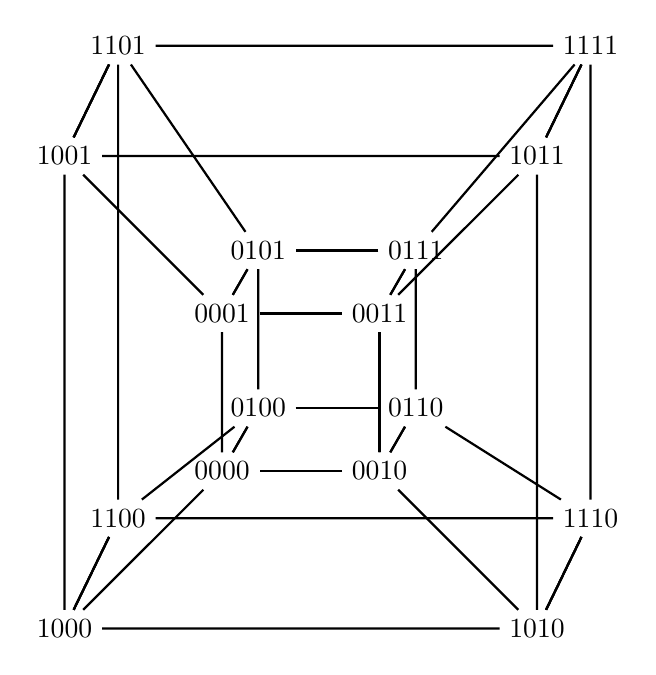
\begin{tikzpicture}[scale=2]
	 \tikzstyle{vertex}=[rectangle]
	 \tikzstyle{edge} = [draw,thick,-,black]
	 \node[vertex] (v0) at (0,0) {$0000$};
	 \node[vertex] (v1) at (0,1) {$0001$};
	 \node[vertex] (v2) at (1,0) {$0010$};
	 \node[vertex] (v3) at (1,1) {$0011$};
	 \node[vertex] (v4) at (0.23, 0.4) {$0100$};
	 \node[vertex] (v5) at (0.23,1.4) {$0101$};
	 \node[vertex] (v6) at (1.23,0.4) {$0110$};
	 \node[vertex] (v7) at (1.23,1.4) {$0111$};
	 \node[vertex] (v8) at (-1,-1) {$1000$};
	 \node[vertex] (v9) at (-1,2) {$1001$};
	 \node[vertex] (v13) at (-0.66,2.7) {$1101$};
	 \node[vertex] (v12) at (-0.66,-0.3) {$1100$};
	 \node[vertex] (v10) at (2,-1) {$1010$};
	 \node[vertex] (v14) at (2.34,-0.3) {$1110$};
	 \node[vertex] (v11) at (2,2) {$1011$};
	 \node[vertex] (v15) at (2.34,2.7) {$1111$};
	 \draw[edge] (v0) -- (v1) -- (v3) -- (v2) -- (v0);
	 \draw[edge] (v0) -- (v4) -- (v5) -- (v1) -- (v0);
	 \draw[edge] (v2) -- (v6) -- (v7) -- (v3) -- (v2);
	 \draw[edge] (v4) -- (v6) -- (v7) -- (v5) -- (v4);
	 \draw[edge] (v8) -- (v9) -- (v13) -- (v12) -- (v8);
	 \draw[edge] (v0) -- (v4) -- (v12) -- (v8) -- (v0);
	 \draw[edge] (v1) -- (v9) -- (v13) -- (v5) -- (v1);
	 \draw[edge] (v2) -- (v10) -- (v14) -- (v6) -- (v2);
	 \draw[edge] (v8) -- (v10) -- (v14) -- (v12) -- (v8);
	 \draw[edge] (v3) -- (v11) -- (v15) -- (v7) -- (v3);
	 \draw[edge] (v10) -- (v11) -- (v15) -- (v14) -- (v10);
	 \draw[edge] (v9) -- (v11) -- (v15) -- (v13) -- (v9);
 \end{tikzpicture}
    \caption{A 4-dimensional Hamming (hyper)cube for 4-bit codewords. Moving along any axis flips a specific bit in the codeword.}
    \label{fig:2}
\end{figure}

\section{Hamming(7,4)}

The Hamming(7,4) code is a cyclic code with a codeword length of $n=7$ and a message length of $k=4$. We work over $R = \mathbb F_2[x]/\langle x^7-1\rangle$, and our generator polynomial is $g = x^3 +x^2+1 \in R$. 

It turns out that this code will have a minimum codeword separation of $d=3$, so we can correct any error with Hamming weight $\left\lfloor \frac{d-1}{2} \right\rfloor = 1$. We can compute our lookup table for the syndromes:

\begin{table}[H]
    \centering
    \def\arraystretch{1.7} %  1 is the default, change whatever you need
    \begin{tabular}{r |c|c|c|c|c|c|c|c}

         Error $e(x)$ & $0$ & $1$ & $x$ & $x^2$ & $x^3$ & $x^4$ & $x^5$ & $x^6$ \\
         \hline
         Syndrome $\overline{e(x)}^H$ & $0$ & $1$ & $x$ & $x^2$ & $x^2+1$ & $x^2+x+1$ & $x+1$ & $x^2+x$ \\

    \end{tabular}
    \label{tab:hamming74}
\end{table}

    Let's say we want to send $1010$. We multiply our message $m(x) = x^3+x \in R$ by our generator $g(x)$ to obtain $c(x)= x^6+x^5+x^4+x \in R$. Thus, we send $1110010$ as our codeword. However, on the other end, suppose a bit flips and we receive $\mathbf{0}110010$ for $c'(x)=x^5+x^4+x \in R$. Then we can take $H = \{g(x)\}$ and compute $\overline{c'(x)}^H = x^2+x$, and by looking it up in our table we can correctly deduce that the $x^6$ bit flipped. Thus, we recover the original codeword $c(x)=c'(x)+x^6$, and we can recover the original message $x^3+x$ by dividing by $g(x)$. See Appendix for Mathematica code working through this example.

    Note that this formulation of the Hamming(7,4) code might be slightly different than others you may be familiar with. Specifically, one popular formulation of the Hamming(7,4) code is that of appending three parity check bits to the end of our message, but in our formulation, the original message does not necessarily appear as a substring in the encoded codeword. To arrive at the parity-bit formulation, we can use a \emph{systematic encoding} instead of multiplying by the generator: we take $c(x)=x^3 m(x) - \overline{x^3 m(x)}^H$ instead of $c(x) = g(x)m(x)$. This still gives us an injective mapping from polynomials with degree less than $4$ into $\langle g(x)\rangle$, and the relevant properties are preserved for syndrome decoding to still work. For general cyclic codes, this systematic encoding scheme would be \[c(x)= x^{n-k} m(x) - \overline{x^{n-k}m(x)}^H.\] Fun exercise for the reader to show this also works.

    We can work through the $m(x)=x^3+x$ example again: we have $\overline{x^3 m(x)}^H =1$ so $c(x) = x^6+x^4+1$. We have encoded $1010$ into $1010\underline{001}$, appending these three parity bits to our message. Say we flip the first bit into $\mathbf{0}010001$, then we have $c'(x) = x^4+1$, and $\overline{c'(x)}^H = x^2+x$. Looking that syndrome up in our table, we find correctly that the $x^6$ bit was flipped.

\section{Conclusion}
Error correcting codes are cool! We have seen how cyclic codes naturally correspond to ideals $\langle g \rangle$ in a polynomial ring $R=\mathbb F_2[x] / \langle x^n - 1\rangle$, and how one can use the remainders produced by the division algorithm to correct errors. By calculating the minimum Hamming distance between two codewords, we can guarantee that errors with Hamming weight at or below the threshold of $\left\lfloor \frac{d-1}{2} \right\rfloor$ are correctable.

\newpage{}
\nocite{CoxIVA}
\nocite{CoxUAG}
\printbibliography

\section{Appendix}
\begin{lstlisting}[language=Mathematica]
In[1]:= F2 = FiniteField[2];
In[2]:= g = F2[1] (x^3 + x^2 + 1);
In[3]:= m = F2[1] (x^3 + x);

In[4]:= Table[PolynomialRemainder[F2[1] x^i, g, x], {i, 0, 6}] /. 
 F2[1] -> 1
Out[4]= {1, x, x^2, 1 + x^2, 1 + x + x^2, 1 + x, x + x^2}

In[5]:= (c = m*g // ExpandAll) /. F2[1] -> 1
Out[5]= x + x^4 + x^5 + x^6

In[6]:= (cr = c + F2[1] x^6) /. {F2[1] -> 1, F2[0] -> 0}
Out[6]= x + x^4 + x^5

In[7]:= PolynomialRemainder[cr, g, x] /. F2[1] -> 1
Out[7]= x + x^2

In[8]:= (F2[1]*PolynomialReduce[cr + F2[1] x^6, g, x] // 
   ExpandAll) /. {F2[1] -> 1, F2[0] -> 0}
Out[8]= {{x + x^3}, 0}

In[9]:= (* Demonstration of systematic encoding *)
(PolynomialRemainder[x^3 m, g, x] // ExpandAll) /. F2[1] -> 1
Out[9]= 1

In[10]:= (x^3 m - PolynomialRemainder[x^3 m, g, x] // ExpandAll) /. 
 F2[1] -> 1
Out[10]= 1 + x^4 + x^6

In[11]:= PolynomialRemainder[F2[1] (1 + x^4), g, x] /. F2[1] -> 1
Out[11]= x + x^2
\end{lstlisting}

\section{Bonus Content}

The \emph{Singleton bound}: $d \le n-k+1$.

Really cool problem from Cox, Little, O'Shea (\emph{Using Algebraic Geometry} Chapter 9 \S3 Exercise 10): Reed Solomon codes are low pass filters, as $\varphi : \mathbb F_q[x] /\langle x^{q-1}-1\rangle \to \mathbb F_q^{q-1}$ given by evaluating the polynomial at powers of the primitive element is the Fourier transform??

\end{document}